\chapter{背景:ニューラルネットワーク}

本章では、教師あり学習とMLPの説明を行った後、MLPの応用例であるCNN及びGANを紹介する。そして、これらの応用例を組み合わせたPix2pixを紹介する。

\section{教師あり学習}

教師あり学習は機械学習の手法の一つである。機械学習とは、学習データと呼ばれるデータに含まれる特徴をコンピュータプログラム~(モデル)~が自動で学習し、学習したモデルを用いて何らかの問題を解く手法のことである。また、教師あり学習では、説明変数と対応するべき目的変数のペアとして学習データが与えられる。

\subsection{教師あり学習の目的}

$X,Y$をそれぞれ説明変数と目的変数の空間とすると、$f:X\rightarrow Y$のうち任意の$\boldsymbol{x} \in X$について正しい値を出力する関数$f^{'}$を表現するモデルを作成することが教師あり学習の目的である。また、$\boldsymbol{x} \in X$について、$f(\boldsymbol{x})$の$f^{'}(\boldsymbol{x})$への近似の程度を評価する関数を損失関数$L$と呼ぶ。よって、損失関数は$\mathbb{R}^+$を非負の実数として$L:Y \times Y \rightarrow \mathbb{R}^+$と定義でき、値が小さいほど近似の程度が良い。

\subsection{教師あり学習モデルの学習と汎化}

任意の$\boldsymbol{x} \in X$と対応する$\boldsymbol{y} \in Y$の組を用意することは現実的には難しいため、学習データはランダムに抽出されているという仮定のもとにある。この時、学習データに含まれる任意の説明変数$\boldsymbol{x}$について損失関数$L$の値の期待値を小さくするように学習を行う。すなわち、目的関数は式\ref{eq:SL1}となる。

\begin{align}
    \label{eq:SL1}
    \hat{f}=\argmin _{f} \mathbb{E}[L(\boldsymbol{y},f(\boldsymbol{x}))]
\end{align}

また、$\hat{f}$はモデルの学習結果であるが、学習データに含まれる説明変数のみで最適であるため、$\hat{f}$は$f^{'}$に一致するとは限らない。したがって、学習データとは別に評価データを用意し、モデルの評価データに対する性能~(汎化性能)~を測定する必要がある。

%機械学習は、教師あり学習、教師なし学習、強化学習、の三つに主に分類することができる。
%教師あり学習とは、学習データにおいて入力値に対応する出力値がわかる機械学習の手法である。また、出力値が離散値である問題を分類問題と呼び、出力値が連続値である問題を回帰問題と呼ぶ。
%教師なし学習とは、学習データにおいて入力値に対応する出力値がわからない機械学習の手法である。例としては、データ内で類似したもの同士をまとめるクラスタリングがあげられる。
%強化学習とは、報酬を最大化させるために特定の状況での適切なアクションを選択する機械学習の手法である。

\section{MLP}

MLP~(Multilayer~perceptron)~はニューラルネットワークの一つであり、教師あり学習の手法として用いられる。

\subsection{ニューラルネットワーク}

ニューラルネットワークは、神経細胞と神経細胞間のシナプス結合を通る電気信号により実現される脳の機能に類似した数理モデルである。ニューラルネットワークでは、神経細胞を人工ニューロンとして表現し、シナプス結合の強度を人工ニューロン間の重みとして表現する。

\subsection{人工ニューロンの構造と定式化}
\label{subsec:neuron}
%バイアス項の説明

\begin{figure}[b]
\begin{center}
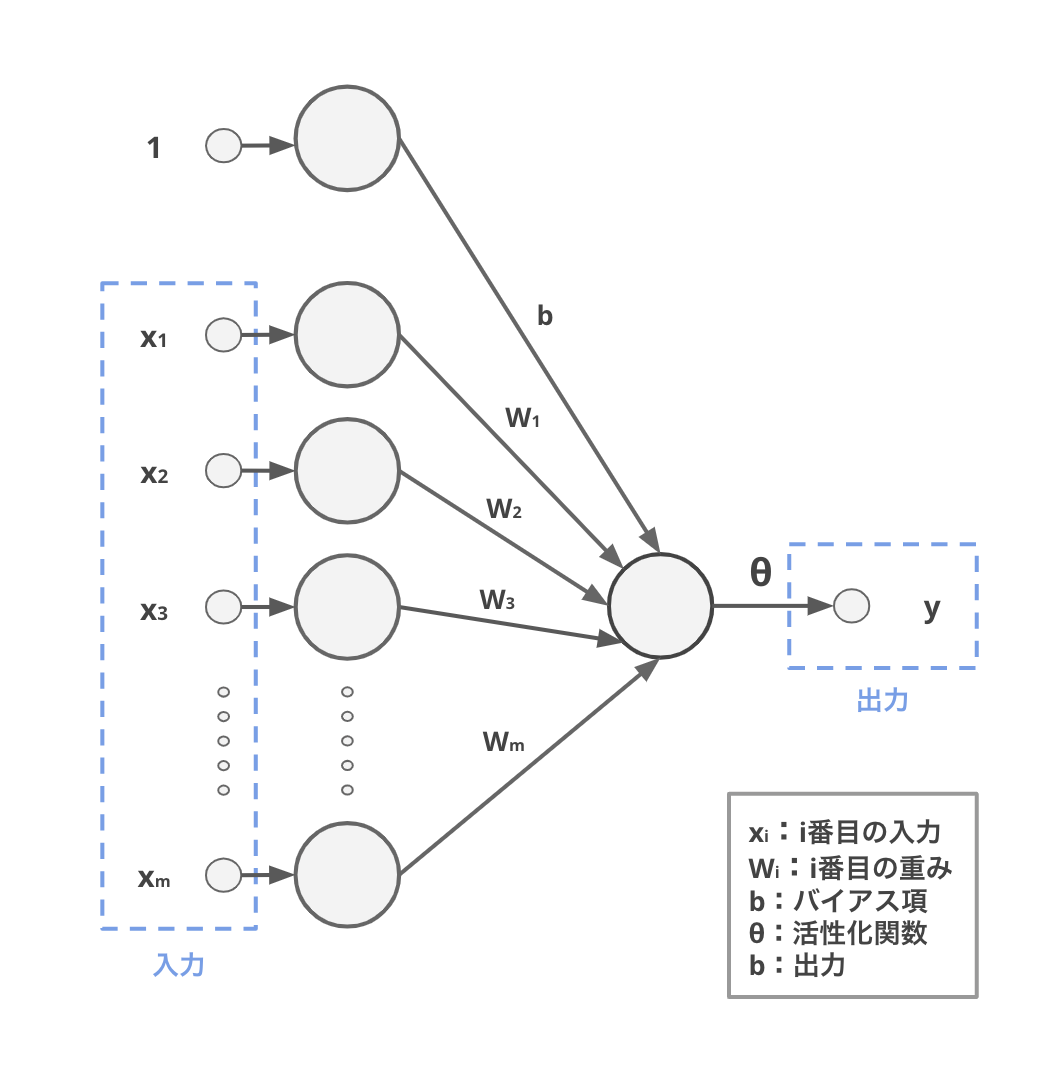
\includegraphics[width=0.7\hsize]{figure/neuron.png}
\caption{人工ニューロン}
\label{fig:neuron}
\end{center}
\end{figure}

MLPにおける人工ニューロンは図\ref{fig:neuron}のように$m$個の入力$x_i$に対応した重み$w_i$をかけた重み付き和に対して活性関数$\theta$を作用させた出力$y$を返す。つまり、式\ref{eq:MLP0_0}として定式化される。

\begin{align}
    \label{eq:MLP0_0}
    \boldsymbol{y}=\theta(\sum_{i=1}^{m} W_{i} \times \boldsymbol{x_i})
\end{align}

また、活性化関数としては出力値を調整するために適当な関数が選ばれる。多くの場合は式\ref{eq:ReLU}のReLU関数や式\ref{eq:Sigmoid}のSigmoid関数などの非線形関数が用いられる。

\begin{align}
    \label{eq:ReLU}
    \theta_{ReLU}(x)&=max(0,x)\\
    \label{eq:Sigmoid}
    \theta_{Sigmoid}(x)&=\frac{1}{1+e^{-x}}
\end{align}

\subsection{MLPの構造と定式化}

\begin{figure}[b]
\begin{center}
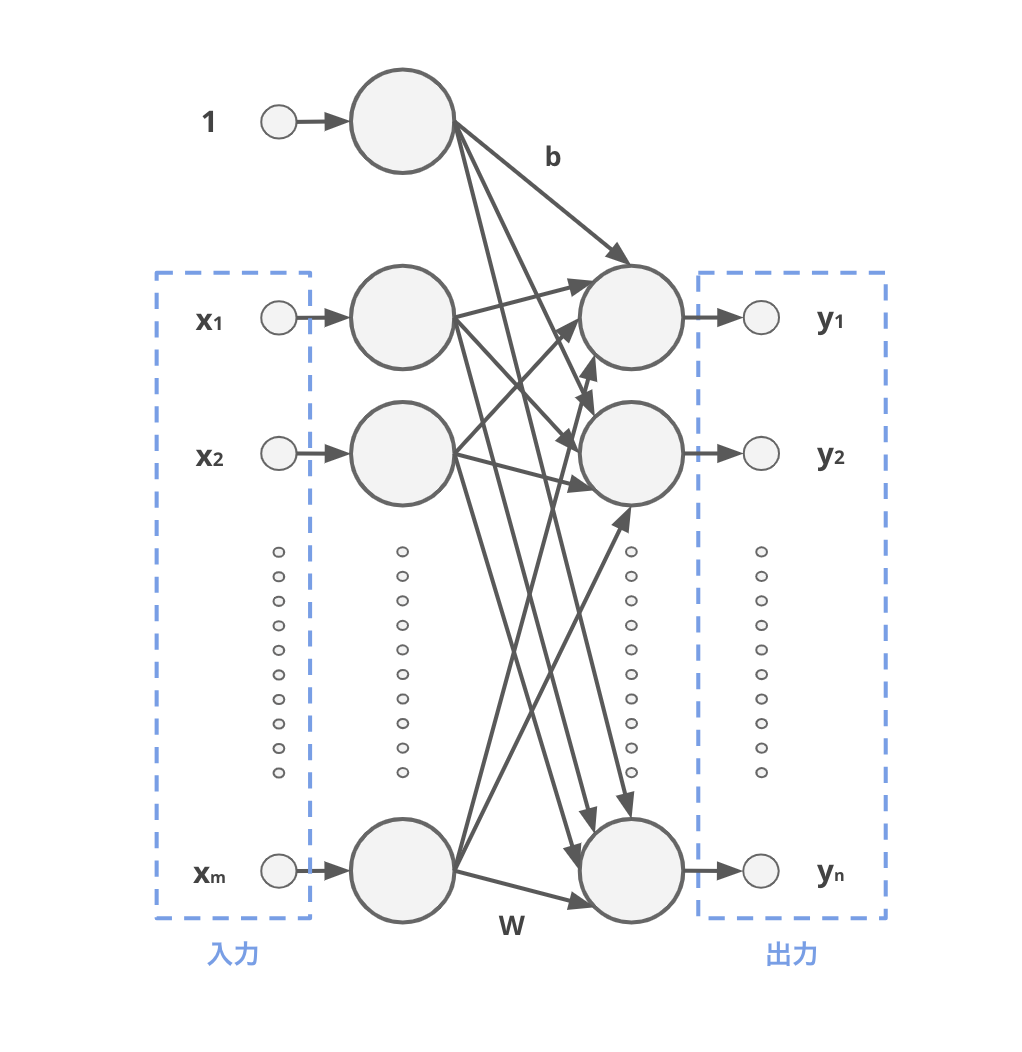
\includegraphics[width=0.6\hsize]{figure/mlp_net0.png}
\caption{MLPの一層}
\label{fig:MLP_net0}
\end{center}
\end{figure}

MLPの構成単位は、\ref{subsec:neuron}節の人工ニューロンが複数並んだ層である~(図\ref{fig:MLP_net0})~。この層の出力$\boldsymbol{y}$は式\ref{eq:MLP0_0}より式\ref{eq:MLP0_1}として導出できる。また、$\boldsymbol{x} \mapsto W\boldsymbol{x}+\boldsymbol{b}$はアフィン変換と呼ばれ、$\theta$は活性化関数である。

\begin{align}
    \label{eq:MLP0_1}
    \boldsymbol{y}&=\theta(W\boldsymbol{x}+\boldsymbol{b})
\end{align}

ここで、$\boldsymbol{x}$は層の入力となる実ベクトル、$\boldsymbol{y}$は層の出力となる実ベクトル、$\boldsymbol{b}$は第$i$成分が$i$番目の出力に対応したバイアス項となる実ベクトル、$W$は$(i,j)$成分が$i$番目の人工ニューロンと$i$番目の出力に対応した重みとなる実ベクトル、である。

\begin{figure}[b]
\begin{center}
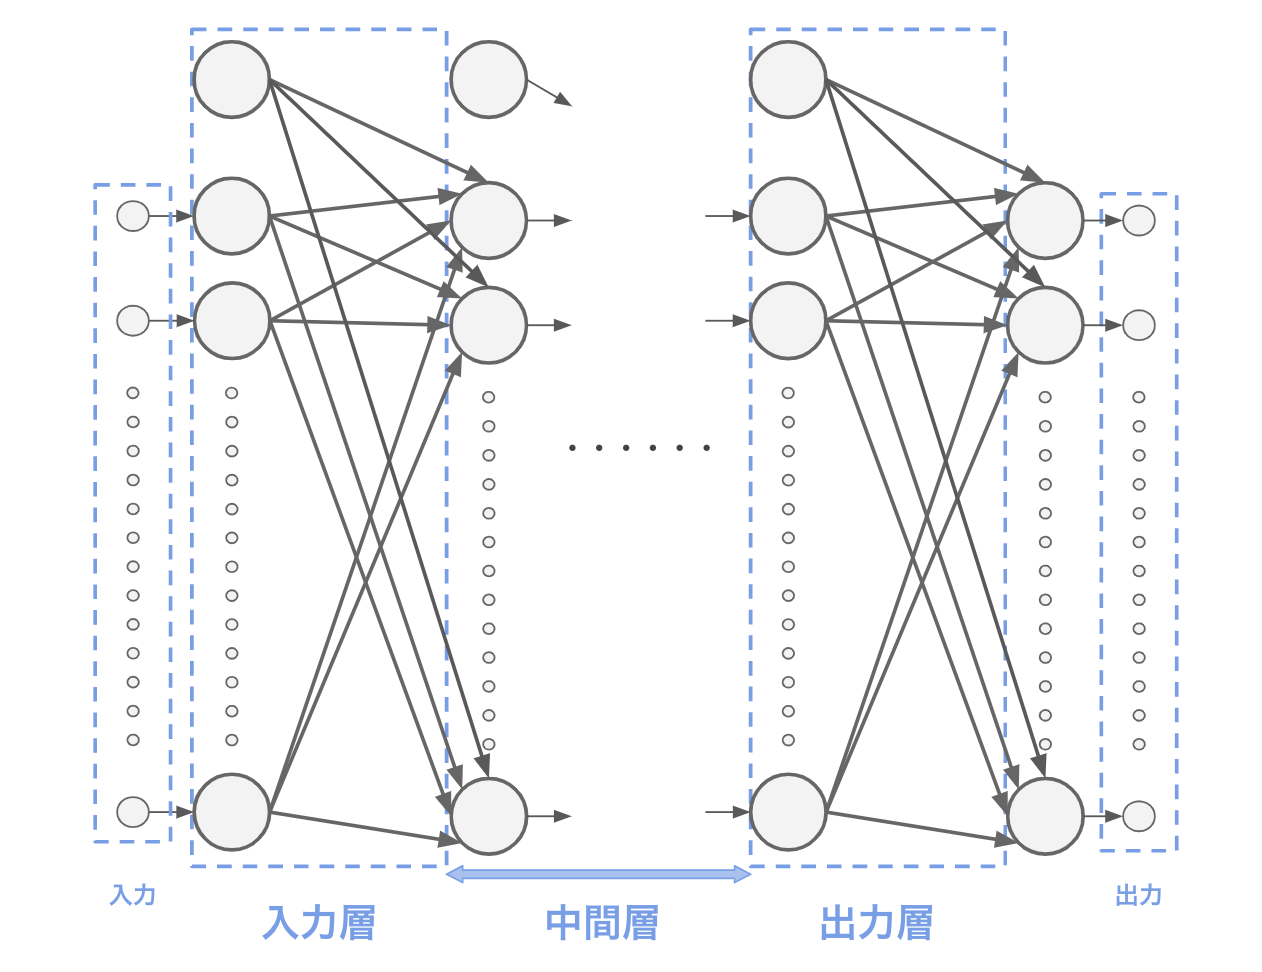
\includegraphics[width=0.8\hsize]{figure/mlp_net1.png}
\caption{MLPのネットワーク}
\label{fig:MLP_net1}
\end{center}
\end{figure}

MLPは、図\ref{fig:MLP_net0}を一層とした順伝播型の階層構造のニューラルネットワークである~(図\ref{fig:MLP_net1})~。一層ずつの入力層と出力層、その間の中間層から構成される。層を構成する人工ニューロンの出力は次の層の全ての人工ニューロンに渡されるため、MLPを構成する層を全結合層とも呼ぶ。また、$n$を層数とおけば、MLPは式\ref{eq:MLP0_2}として定式化される。

\begin{align}
    \label{eq:MLP0_2}
    \hat{f}(\boldsymbol{x})&=\theta_{n}(W_{n}(\theta_{n-1}(W_{n-1}\cdots(\theta_{1}(W_{1}\boldsymbol{x}+\boldsymbol{b_{1}}))\cdots+\boldsymbol{b_{n-1}}))+\boldsymbol{b_{n}})
\end{align}

ここで、$\boldsymbol{x}$は実ベクトル、$\theta_{i}$は$i$番目の活性化関数、$W_{i}$は$i$番目の行列、$\boldsymbol{b_{i}}$は$i$番目の実ベクトル、である。

\subsection{MLPの学習}

%誤差逆伝播

MLPでは、学習により任意の$i$で$W_i,\boldsymbol{b_i}$を適切に定める必要がある。また、教師あり学習では損失関数を減少させる方向に学習は進むため、それぞれ式\ref{eq:MLP2_0}と\ref{eq:MLP2_1}にしたがって$W_i,\boldsymbol{b_i}$は更新される~(勾配降下法)~。

\begin{align}
    \label{eq:MLP2_0}
    W _i &\leftarrow W_i - \eta \frac{d L}{dW_i} \\
    \label{eq:MLP2_1}
    \boldsymbol{b _i} &\leftarrow \boldsymbol{b_i} - \eta \frac{d L}{dW_i}
\end{align}

%Adam,SGDの原著論文に目を通す
ここで、$\eta$は任意の正の実数であり、学習率と呼ばれる。なお、損失関数としては式\ref{eq:MLP3}の平均二乗誤差$L_{MSE}$や式\ref{eq:MLP4}の平均絶対誤差$L_{MAE}$などが用いられる。また、学習率を適切に設定する最適化アルゴリズムとして、Stochastic~Gradient~Descent~\cite{SGD}やAdam~\cite{Adam}などが用いられる。

\begin{align}
    \label{eq:MLP3}
    L_{MSE}&=\frac{1}{n}\sum _{j} {(\boldsymbol{y_j} - \hat{f}(\boldsymbol{x_j})^2}\\
    \label{eq:MLP4}
    L_{MAE}&=\frac{1}{n}\sum _{j} {|\boldsymbol{y_j} - \hat{f}(\boldsymbol{x_j})|}
\end{align}

\section{CNN}

%内容確認、図を作る

CNN~(Convolution~Neural~Network)~は主に画像認識の分野で成果を残している代表的な順伝播型ニューラルネットワークである~\cite{AlexNet}。CNNのネットワーク構造はMLPにおいて全結合層を脳の視覚野の構造を模倣するように置換したものとみなせる。また、脳の視覚野では、刺激の位置により異なったニューロンの活動電位が発生し、受容する情報の特徴によって受容野が階層構造を形成している~\cite{neocognition}。つまり、CNNは、人工ニューロン間の結合が局所領域に限定され、層ごとに受容する情報が異なるニューラルネットワークである。具体的には、画像の局所領域の特徴量を抽出する畳み込み層と局所領域の特徴量をまとめるプーリング層~(サブサンプリング層)~を繰り返した構造である~\cite{CNNsurvey}。また、以下では画像~(二次元データ)~でCNNの説明を行うが、他の次元のデータについても同様の説明を行うことができる。

\subsection{畳み込み層}

\begin{figure}[b]
\begin{center}
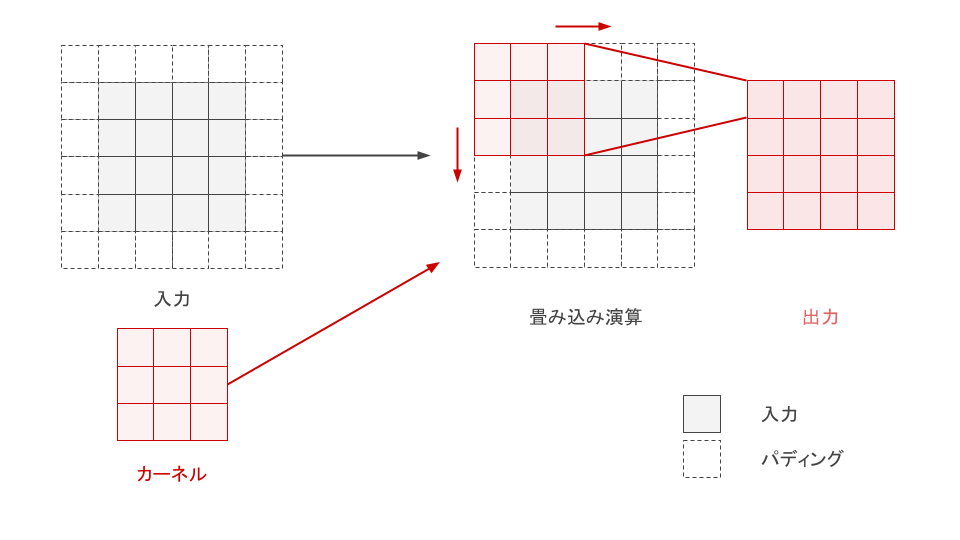
\includegraphics[width=\hsize]{figure/convolution.png}
\caption{畳み込み層}
\label{fig:conv}
\end{center}
\end{figure}
    

畳み込み層においては、図\ref{fig:conv}のようにカーネルと呼ばれるフィルターを用いて畳み込み演算を行う。畳み込み演算ではカーネルのそれぞれの値を重みと見た重み付き和の計算が行われる。また、カーネルは予め決めた幅~(ストライド)~によって移動させる。そして、そのまま畳み込み演算を行った場合は特徴量マップが元の画像より小さいサイズとなるため、一般には元の画像の周りに適当な幅で値を埋める操作を行う~(パディング)~。また、カーネルサイズを$ks$、ストライド幅を$st$、パディング数を$pad$、入力サイズを$in$、出力サイズを$out$、とした時、式\ref{eq:conv}が成り立つ。

\begin{align}
    \label{eq:conv}
\end{align}

加えて、異なるカーネルが複数あっても良く、カーネルが複数あるときは出力する特徴量マップの数はその数になる。入力のチャンネル数が1でない場合もそれぞれのチャンネルで求めた畳み込み演算の値を足したものが返される。

\subsection{プーリング層}

\begin{figure}[b]
\begin{center}
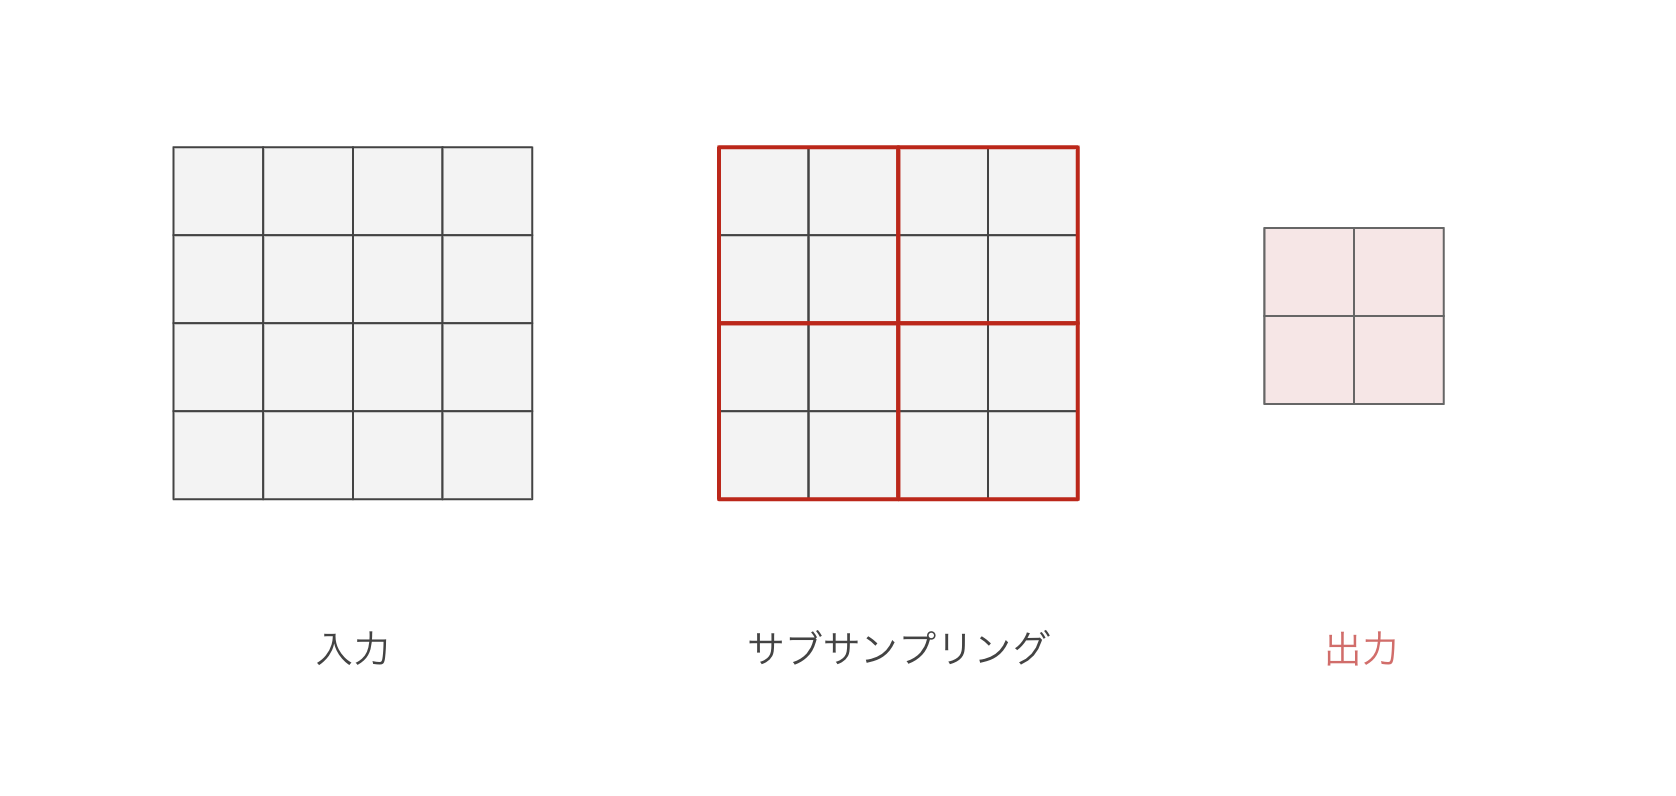
\includegraphics[width=\hsize]{figure/pooling.png}
\caption{プーリング層}
\label{fig:pooling}
\end{center}
\end{figure}

プーリング層においては、図\ref{fig:pooling}のように情報量を圧縮する~(サブサンプリング、ダウンサンプリング)~。入力を局所領域ごとに分解し、その局所領域ごとに何らかの操作を行う。この操作が最大値をとる場合はMax~Pooling、平均値をとる場合はAverage~Poolingと呼び、主にこの二つがプーリング層としては用いられる。

\subsection{CNNの利点}

CNNにはMLPと比べて主に二つの利点がある~\cite{CNNsurvey}。一つ目は、パラメータ数が減少する点である。全結合層の場合は入力の数と出力の数の積が層のパラメータ数となるが、畳み込み層においてはカーネルに含まれるパラメータ数のみが層のパラメータ数となるため、パラメータ数が減少する。また、プーリング層においてもサブサンプリングにより特徴量マップのサイズが小さくなるためパラメータ数の減少に寄与する。二つ目は、様々な解像度での特徴を取得できる点である。プーリング層によりサブサンプリングをすることで解像度が低下し、異なるスケールでの隣接する特徴の共起を得ることができると期待される。

\section{GAN}

\begin{figure}[b]
\begin{center}
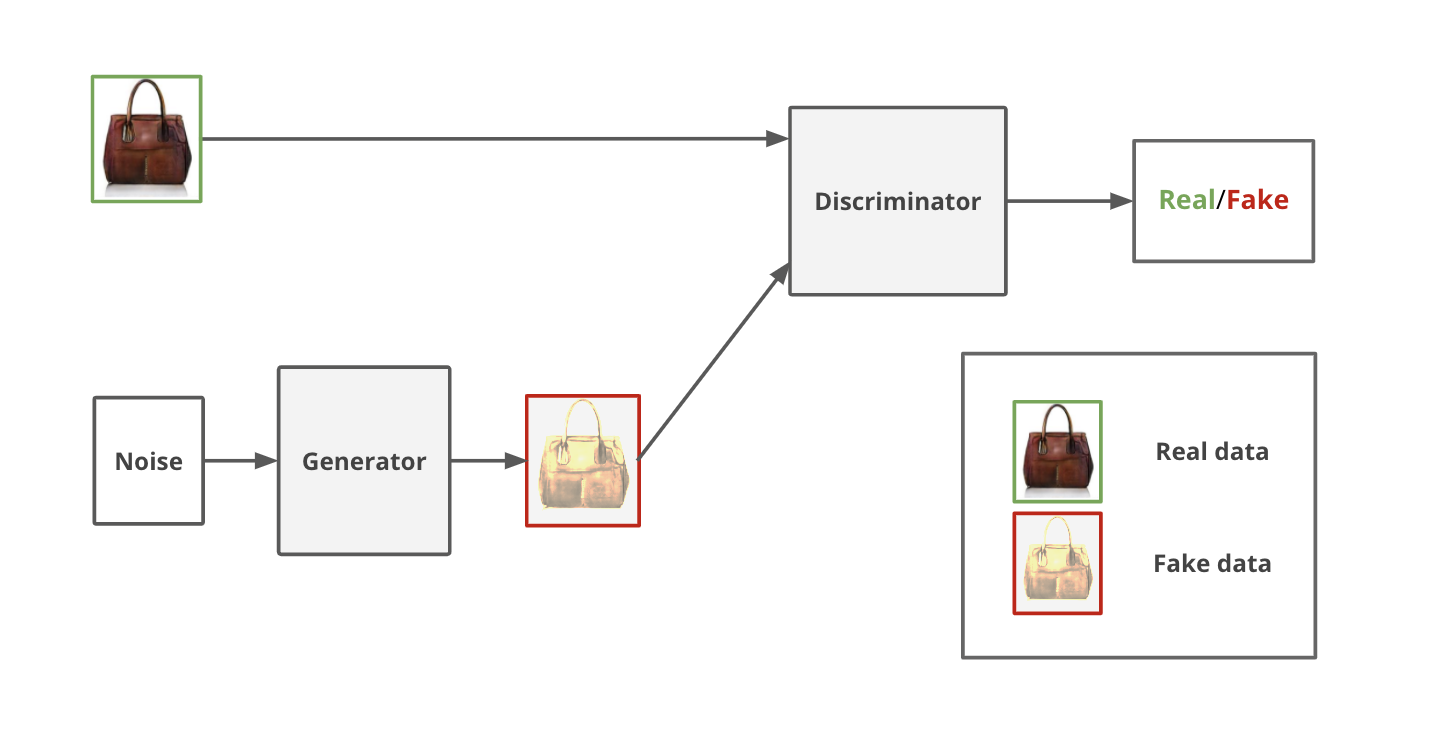
\includegraphics[width=\hsize]{figure/GAN_net.png}
\caption{GANのネットワーク\\
図は文献~\cite{pix2pix}のFigure~1を用いて作成した。}
\label{fig:GAN_net}
\end{center}
\end{figure}

GAN~(Generative~Adversarial~Networks)~\cite{GAN}はニューラルネットワークの応用例であり、学習データの特徴を持つ擬似的なデータを生成することを目指す手法である。この手法は実在しないアイドルの写真を生成する際などに用いられる~\cite{idol}。また、GANは図\ref{fig:GAN_net}のように二つのニューラルネットワークで構成され、それぞれのネットワークはDiscriminator~(識別モデル)~とGenerator~(生成モデル)~と呼ばれる。

\subsection{GANの学習}

生成モデルと識別モデルの二つのネットワークはランダムに初期化された後に競合的に学習を進める。まず、識別モデルはデータがFake~data~(生成モデルの出力)~とReal~data~(学習データ)~のどちらであるかを識別できるように学習を進める。そして、生成モデルは識別モデルが学習データであると誤って識別するように、Noise~(ノイズ)~を元に学習データに近いデータを出力する。この二つの学習を交互に繰り返すことで、漸進的に生成モデルが学習データにより近いデータを生成できるようになると期待される。また、ノイズは適当な次元の実ベクトルであり、生成モデルの出力の揺らぎを表現する潜在変数の役割を果たす。

\subsection{GANの定式化}

GANでは、生成モデルの目的関数は式\ref{eq:GAN_G}、識別モデルの目的関数は式\ref{eq:GAN_D}として定式化される。

\begin{align}
    \label{eq:GAN_G}
    \argmin _{\theta_G}& \mathbb{E}_{\boldsymbol{z}}[\log (1-D(G(\boldsymbol{z};\theta_G);\theta_D))]\\
    \label{eq:GAN_D}
    \argmax _{\theta_D}& \mathbb{E}_{\boldsymbol{x}}[\log D(\boldsymbol{x};\theta_D)]+\mathbb{E}_{\boldsymbol{z}}[\log (1-D(G(\boldsymbol{z};\theta_G);\theta_D))]
\end{align}


ここで、$\boldsymbol{x}$は学習データ、$\boldsymbol{z}$は生成モデルへの入力のノイズ、$G(\boldsymbol{z};\theta_G)$はノイズ$\boldsymbol{z}$を入力とする生成モデル、$D(\cdot;\theta_D)$は識別モデル、$\theta_G$は生成モデル$G$のパラメータ、$\theta_D$は識別モデル$D$のパラメータ、である。

\section{Pix2pix}

\begin{figure}[b]
\begin{center}
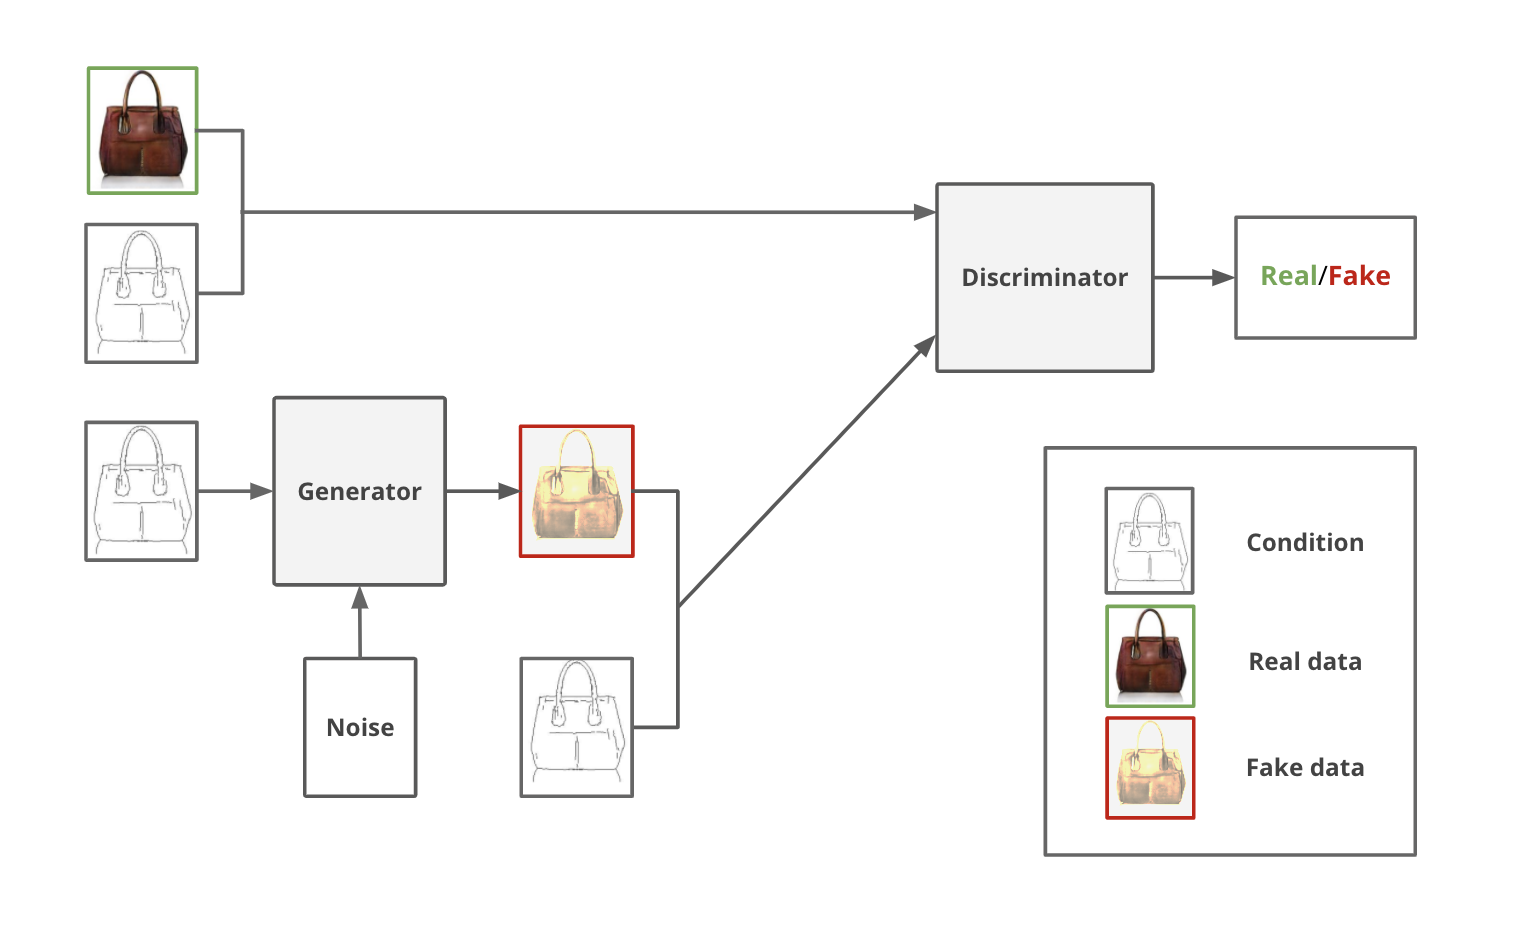
\includegraphics[width=\hsize]{figure/pix2pix_net.png}
\caption{Pix2pixのネットワーク\\
図は文献~\cite{pix2pix}のFigure~1を用いて作成した。}
\label{fig:pix2pix_net}
\end{center}
\end{figure}

\begin{figure}[t]
\begin{center}
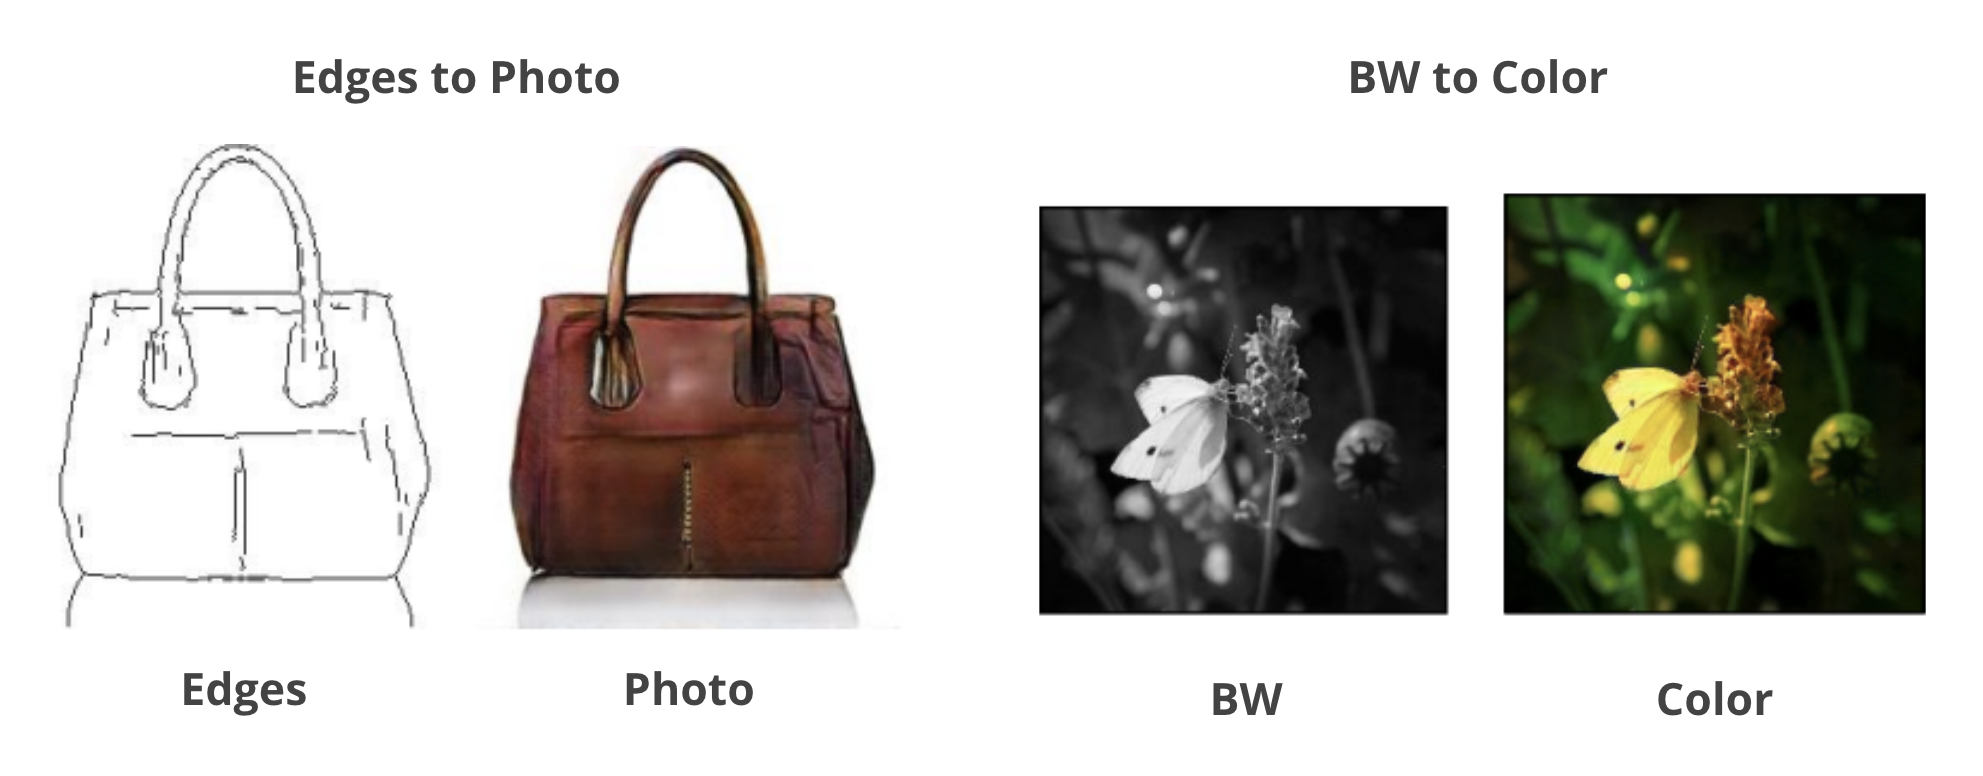
\includegraphics[width=\hsize]{figure/pix2pix_img.png}
\caption{Pix2pixのスタイル変換の例\\
図は文献~\cite{pix2pix}のFigure~1を用いて作成した。}
\label{fig:pix2pix_img}
\end{center}
\end{figure}

Pix2pix~\cite{pix2pix}は、図\ref{fig:pix2pix_net}のようにネットワークの入力に変換元の画像を~Condition~(条件)~として与えることで画像の変換を行うGANである。特定の条件をネットワークの入力に与えるGANとしてはConditional~GAN~(CGAN)~\cite{CGAN}が初めて考案されたが、Pix2pixは与えられた条件画像の構造を維持したまま変換するという点でCGANとは異なる。具体的には、図\ref{fig:pix2pix_img}のように線画から写真への変換や白黒画像からカラー画像への変換を行うことができる。

\subsection{Pix2pixの定式化}

そして、Pix2pixにおいては、生成モデルの目的関数は式\ref{eq:pix2pix_G}、識別モデルの目的関数は式\ref{eq:pix2pix_D}として定式化される。

\begin{align}
    \label{eq:pix2pix_G}
    \argmin _{\theta_G}& \mathbb{E}_{\boldsymbol{y}, \boldsymbol{z}}[\log (1-D(\boldsymbol{y}, G(\boldsymbol{y}, \boldsymbol{z}; \theta_G); \theta_D))]+\mathbb{E}_{\boldsymbol{x}, \boldsymbol{y}, \boldsymbol{z}}[\|\boldsymbol{x}-G(\boldsymbol{y}, \boldsymbol{z}; \theta_G)\|_{1}]\\
    \label{eq:pix2pix_D}
    \argmax _{\theta_D}& \mathbb{E}_{\boldsymbol{x}, \boldsymbol{y}}[\log D(\boldsymbol{x}, \boldsymbol{y}; \theta_D)]+\mathbb{E}_{\boldsymbol{y}, \boldsymbol{z}}[\log (1-D(\boldsymbol{y}, G(\boldsymbol{y}, \boldsymbol{z}; \theta_G); \theta_D))]
\end{align}

ここで、$\boldsymbol{x}$は変換先の学習データ、$\boldsymbol{y}$は変換元の学習データ、$\boldsymbol{z}$は生成モデルへの入力のノイズ、$G(\boldsymbol{y},\boldsymbol{z};\theta_G)$は$\boldsymbol{y}$を条件としノイズ$\boldsymbol{z}$を入力とする生成モデル、$D(\boldsymbol{y},\cdot;\theta_D)$は$\boldsymbol{y}$を条件とする識別モデル、$\theta_G$は生成モデル$G$のパラメータ、$\theta_D$は識別モデル$D$のパラメータ、である。

\subsection{Pix2pixの生成モデル}

\begin{figure}[b]
\begin{center}
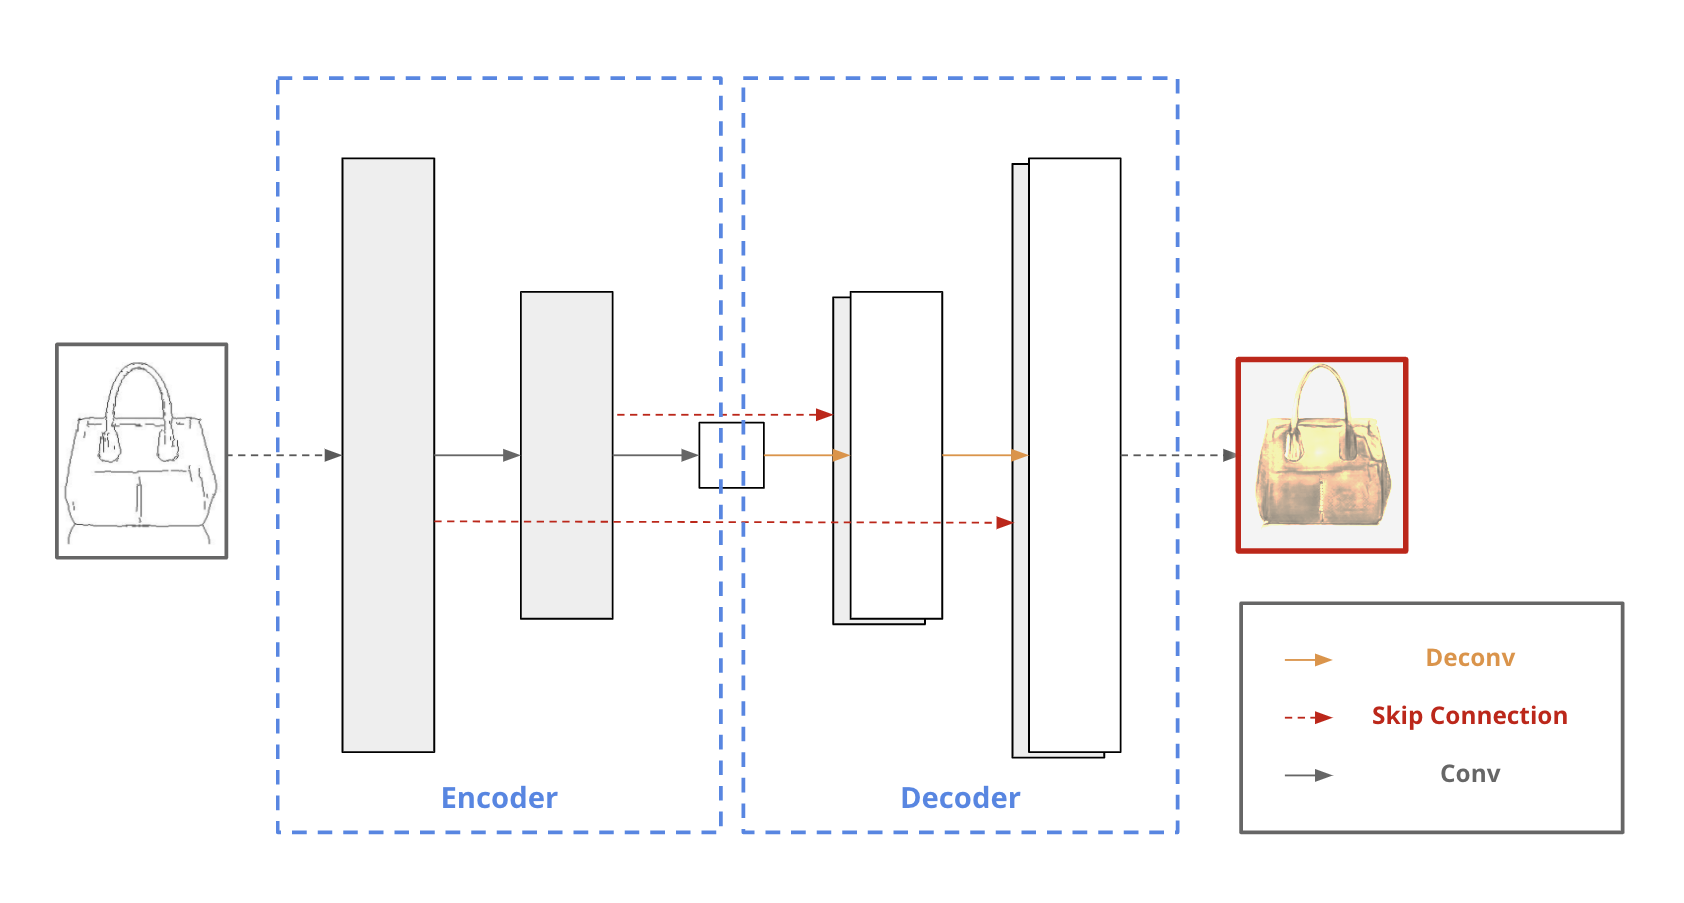
\includegraphics[width=0.8\hsize]{figure/u-net.png}
\caption{生成モデルのネットワーク\\
図は文献~\cite{pix2pix}のFigure~1とFigure~3を用いて作成した。}
\label{fig:u-net}
\end{center}
\end{figure}

Pix2pixの生成モデルには、図\ref{fig:u-net}のようにEncoder-Decoder型のネットワークが用いられる。ただし、変換元の画像と返還後の画像で共通する基本構造であるピクセルの対応関係を維持するために、スキップコネクションが用いられる。このスキップコネクションはU-net~\cite{u-net}で用いられたものと同様の働きをする。具体的には、エンコード前の特徴量マップをデコード時にも利用しており、この特徴量マップによりピクセルの対応関係が維持されると期待される。

また、ノイズとしては実ベクトルではなくDropout~\cite{Dropout}が用いられる。Dropoutとは、ニューラルネットワークの重みの更新の際にランダムにいくつかの重みを0として無視する手法のことである。

\subsection{Pix2pixの識別モデル}

\begin{figure}[b]
\begin{center}
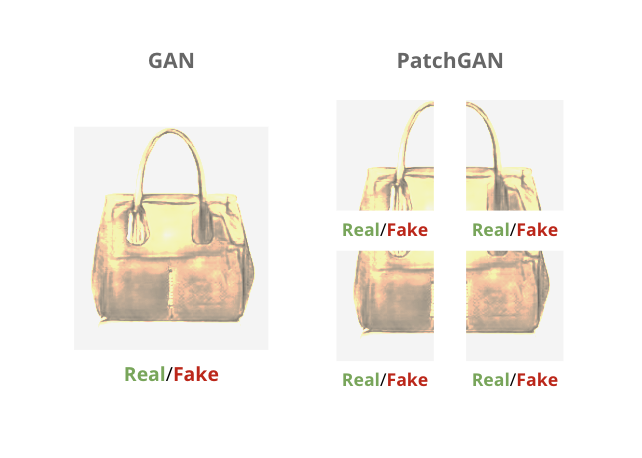
\includegraphics[width=0.6\hsize]{figure/patchgan.png}
\caption{通常のGANとPatchGANの比較\\
図は文献~\cite{pix2pix}のFigure~1を用いて作成した。}
\label{fig:patchgan}
\end{center}
\end{figure}

Pix2pixの識別モデルには、PatchGANという手法が用いられる。PatchGANは図\ref{fig:patchgan}のように画像全体ではなくパッチと呼ばれる局所領域ごとに真偽を求めて平均を出力とする。これにより、局所的な識別精度が高まることが期待される。